\section{Background}
\label{secondchapter}
The sustainable design of structural systems has become more and more salient in recent years due to societal and governmental pressures to reduce greenhouse gas emissions in order to reduce the rate of climate change. Prior research that this paper builds upon focused on reinforced concrete (RC) and timber slabs however there is currently little literature on how slim floor composite slab systems perform in comparison.

To evaluate the sustainability implications of slim floor construction, it is necessary to understand their historical development, structural behaviour, governing design methodologies, and the principles underlying carbon-based optimisation. This literature review therefore examines (i) sustainability in structural design, (ii) the development and typologies of composite slabs and slim floor systems, (iii) current commercial products and design methods according to European standards, and (iv) existing optimisation and design tools incorporating environmental objectives.

The review concludes by identifying limitations in current research and outlining the gap addressed by the present study, namely the integration of slim floor slab cross-sections into a sustainability optimisation tool and the systematic comparison with conventional reinforced concrete flat slabs for multi-storey construction.
%---------------------------------------------------------------
\subsection{Sustainability in Structural Design}
%---------------------------------------------------------------
The construction sector plays a significant role in global greenhouse gas emissions and is therefore central to climate mitigation efforts. According to the \cite{RefWorks:2025brick}, the construction industry accounts for 34\% of carbon dioxide emissions, with cement production alone accounting for 8\% \citep{RefWorks:kaufmann2026stahlbeton}. While operational emissions have reduced in recent decades due to more efficient energy systems, embodied emissions associated with material production have become increasingly dominant in the life-cycle impact of buildings \citep{RefWorks:broyles2024equations}. Embodied carbon refers to greenhouse gas emissions generated during raw material extraction, processing, manufacturing, and construction activities \citep{RefWorks:arnold2025calculate}. The urgency to reduce emissions has led to a growing interest in integrating environmental metrics directly into structural design. Rather than considering sustainability as a secondary assessment performed after design is completed, current research is investigating the impact of conducting environmental evaluations during early-stage decision making.

The environmental performance of structural materials is typically assessed using a Life Cycle Assessment (LCA), which provides a framework for quantifying environmental impacts across different stages of a product’s life cycle. Within the construction sector, LCA methodologies are commonly standardised through environmental product declarations (EPDs), which provide verified environmental impact data for specific building materials. In Europe, Environmental Product Declarations (EPD) follow the ISO 14040 series of international standards and the European Committee for Standardisation EN 15804 standard \citep{RefWorks:arnold2025calculate,RefWorks:del2013lca}. EPDs can be sourced from various places, such as the manufacturer themselves, data sets either representative of a type of product, a region, or based on literature and expert knowledge \citep{RefWorks:2024oekobilanzierung}. LCA commonly distinguishes between life-cycle stages such as raw material extraction and processing (A1), transport to manufacturer (A2), manufacturing (A3), construction processes (A4–A5), use phase (B modules), end-of-life stages (C modules), and benefits and loads beyond the system boundary (D modules) (Figure~\ref{fig:LCAstages}). For early-stage design comparisons, studies often focus on cradle-to-gate (A1–A3) and end of life impacts (C), as these stages account for the majority of embodied emissions in concrete and steel elements and are less sensitive to project-specific assumptions \citep{RefWorks:2024oekobilanzierung}. Global Warming Potential (GWP) is the most widely used environmental impact indicator in structural engineering, measuring the contribution of greenhouse gas emissions to climate change and expressed in kgCO$_{2}$e (kilograms of CO$_2$ equivalent) \citep{RefWorks:2024oekobilanzierung}.

\begin{figure}[h!]
    \centering
    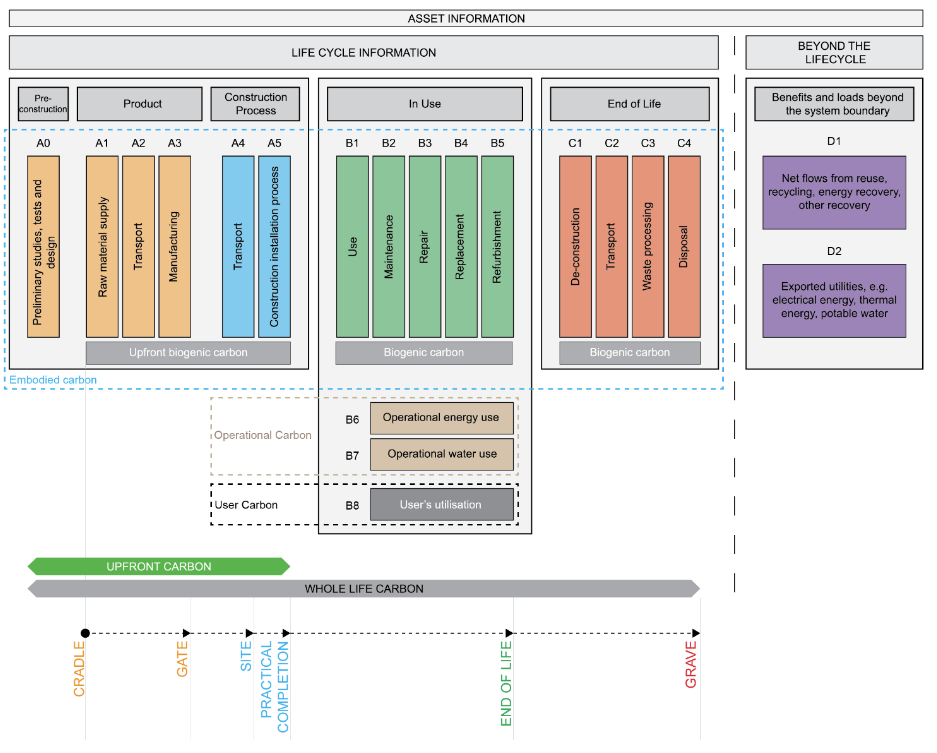
\includegraphics[width=0.7\textwidth]{figures/LCAstages.png}
    \caption{Building and infrastructure life cycle stages and information modules, adopted from \citep{RefWorks:arnold2025calculate}}
    \label{fig:LCAstages}
\end{figure} 

Within multi-storey buildings, floor slabs account for around half of the total concrete volume and 30\% of the total building material \citep{RefWorks:bischof2022fostering}. Due to their repetitive nature and large surface area, even small reductions in slab thickness can result in cumulative material savings. Furthermore, the selected slab system can strongly influence overall structural weight, height, and foundation demand - affecting the environmental performance of the entire building. The choice of slab system therefore has a major influence on the environmental performance of the overall structure. \cite{RefWorks:kaufmann2024white} noted in his white paper, that since the cost of labour has risen significantly, geometrically simple structures (such as flat concrete slabs) have become the most economical option, despite consuming more than double that of the material actually required. Furthermore, solid slabs often have the benefit of functionality since they can easily meet thermal or acoustic requirements and integrate building components with little effort \citep{RefWorks:ammann2024correlations}. \cite{RefWorks:mathern2021addressing} also highlights the increase in steel and concrete use in construction compared to previous buildings of comparable size from decades in the past, similarly due to simple non-optimised solutions as well as more conservative design codes.

Concrete is commonly used due to the fact it is cost effective and durable but as previously stated is a large contributor to greenhouse gas emissions. A significant amount of research has been done to explore opportunities to reduce this impact through the cement mix itself but less focus is put on the impact of efficient and durable load-bearing structures \citep{RefWorks:kaufmann2026stahlbeton}. The greatest potential for emission reductions through efficient design is in the early stages of a project, however the design knowledge of a structure is also at its lowest at this stage \citep{RefWorks:broyles2024equations} (Figure~\ref{fig:designphasegraph}), making it difficult to evaluate the environmental consequences of design decisions.

\begin{figure}[h!]
    \centering
    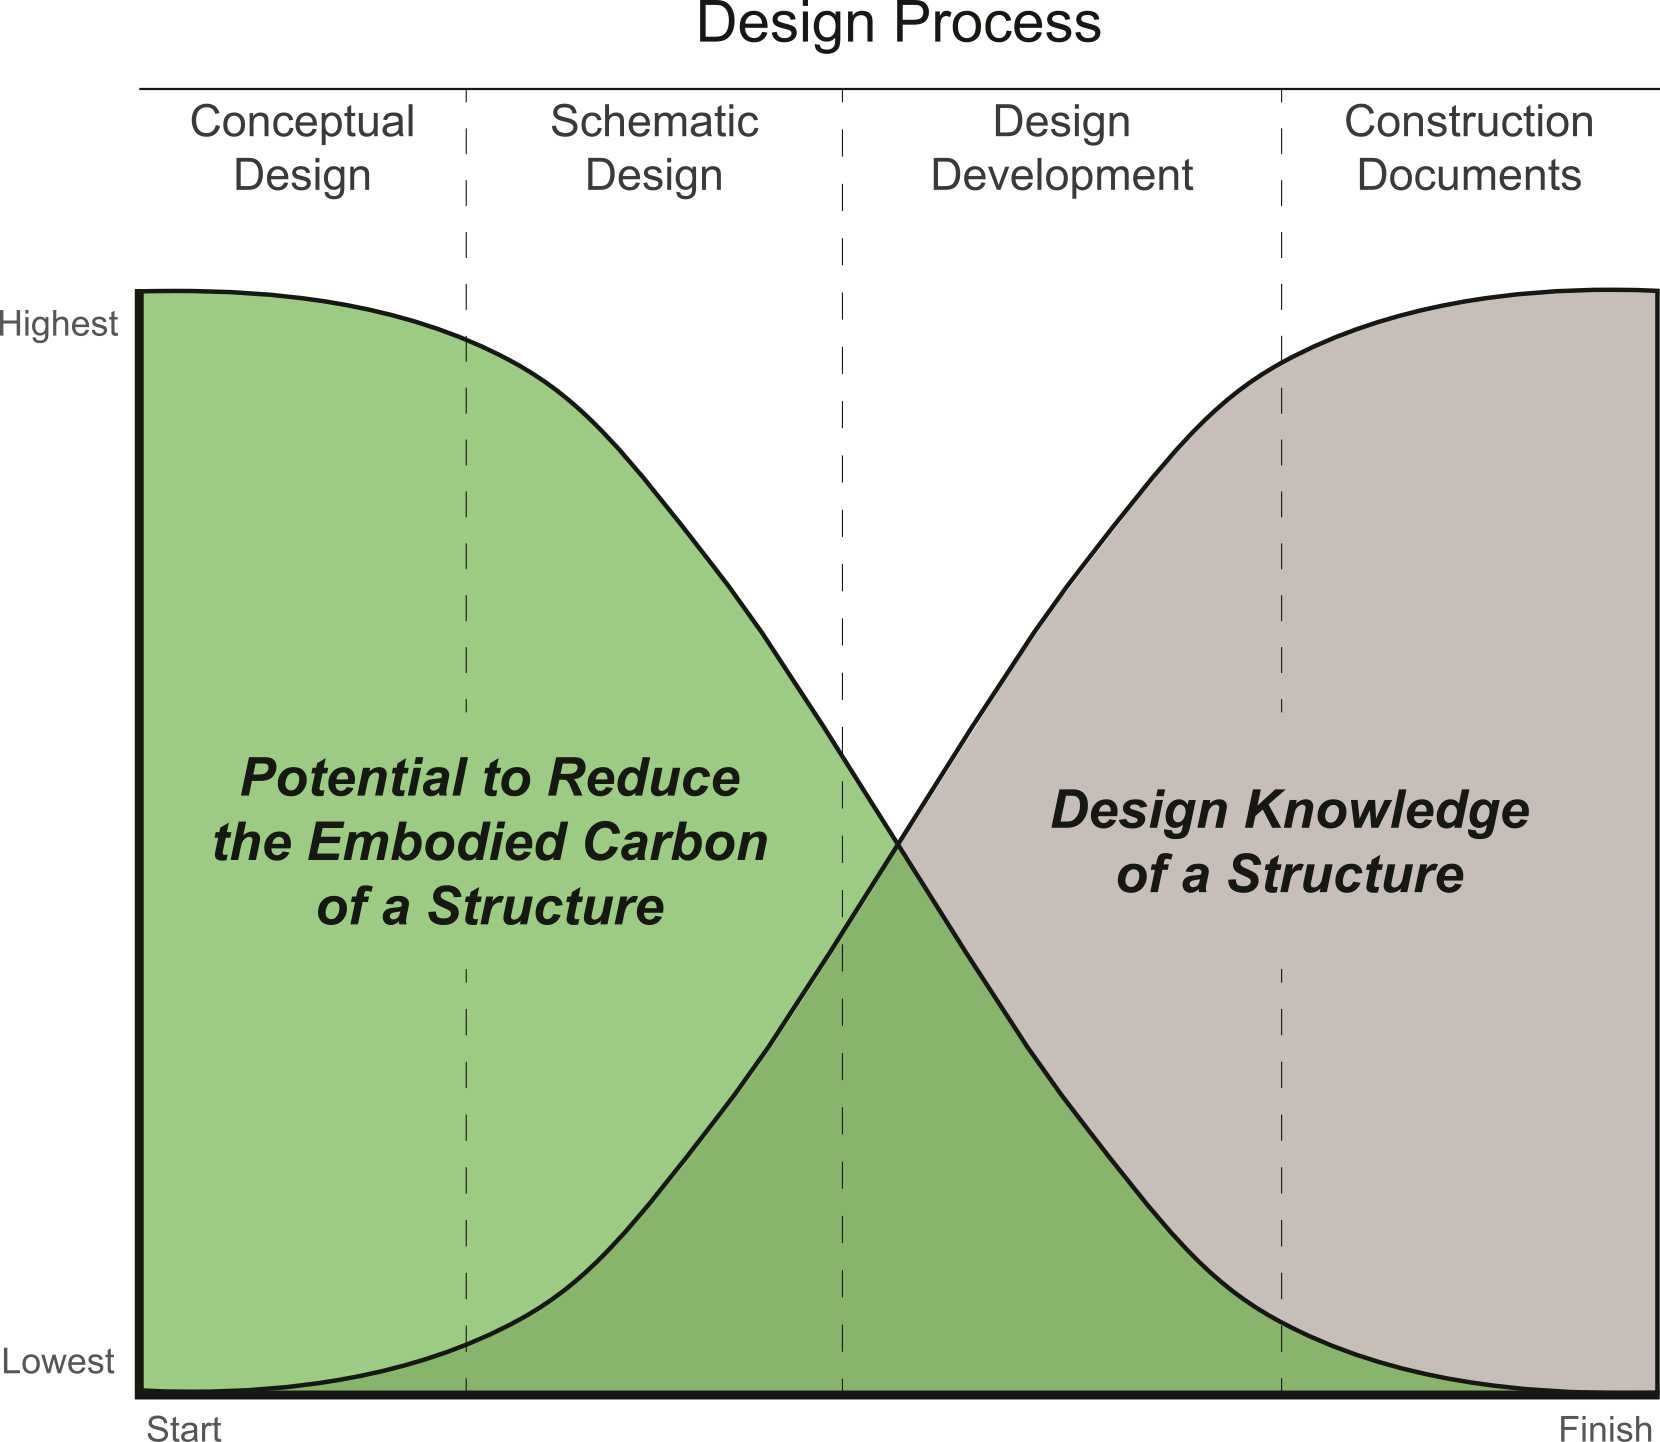
\includegraphics[width=0.7\textwidth]{figures/designphasegraph.jpg}
    \caption{Relationship between reducing the environmental impact of a structure to the design knowledge of a structure during the design process, adopted from  \citep{RefWorks:broyles2024equations}}
    \label{fig:designphasegraph}
\end{figure} 

Traditionally, environmental assessments are conducted post design, based on material quantities extracted from the completed structural designs. However, this approach limits the potential for optimisation, as major design decisions have already been fixed. By embedding GWP into parametric design tools, environmental performance can be evaluated iteratively, allowing GWP to function as an objective within the optimisation process.

According to \cite{RefWorks:broyles2024equations}, a "comprehensive study that establishes EC benchmarks for various concrete floor systems under different design scenarios has not been conducted" - creating difficulty in comparing different concrete systems. In general, research focusing on sustainability driven design is limited, with the scope being narrowed to a specific construction method or on comparing optimisation methods.

\cite{RefWorks:mathern2021addressing} examined a range of optimisation techniques applicable to structural design, including set-based parametric design, multi-objective optimisation, Bayesian optimisation and Kriging surrogate-based optimisation. These approaches had various use cases such as reinforced concrete beams and offshore wind foundations. The main findings were that one should be cautious with results obtained from assessments with few impact categories or that disregard important parts of the works undertaken. 

Recent research has also explored the application of optimisation to floor slab systems. For example, \cite{RefWorks:regulez2022sustainability} compared various slab typologies (including steel-concrete composites) in terms of embodied carbon and span length, with the results concluding that as the span increases the composite slab becomes less efficient than regular RC slabs (Figure~\ref{fig:regulez2022}). The study demonstrated that significant reductions in embodied carbon can be achieved by optimising slab thickness and reinforcement layouts within a parametric design framework. \cite{RefWorks:broyles2024equations} conducted a similar study, analysing 10 concrete floor systems under various design scenarios and span lengths to ascertain their material quantity and embodied carbon. This study focused on a comparison between various RC and PT systems, the results are summarised below in Figure~\ref{fig:broyles2024}. \cite{RefWorks:damico2018accuracy} created a computational tool to minimise steel mass and carbon emissions during early stage design while \cite{RefWorks:ismail2021minimizing} focused on using shape optimisation to minimise embodied energy of RC floor systems in developing countries. Finally, \cite{RefWorks:manmatharasan2025aidriven} examined recent advancements in AI assisted design optimisation in the early design stages.

\begin{figure}[ht]
    \centering
    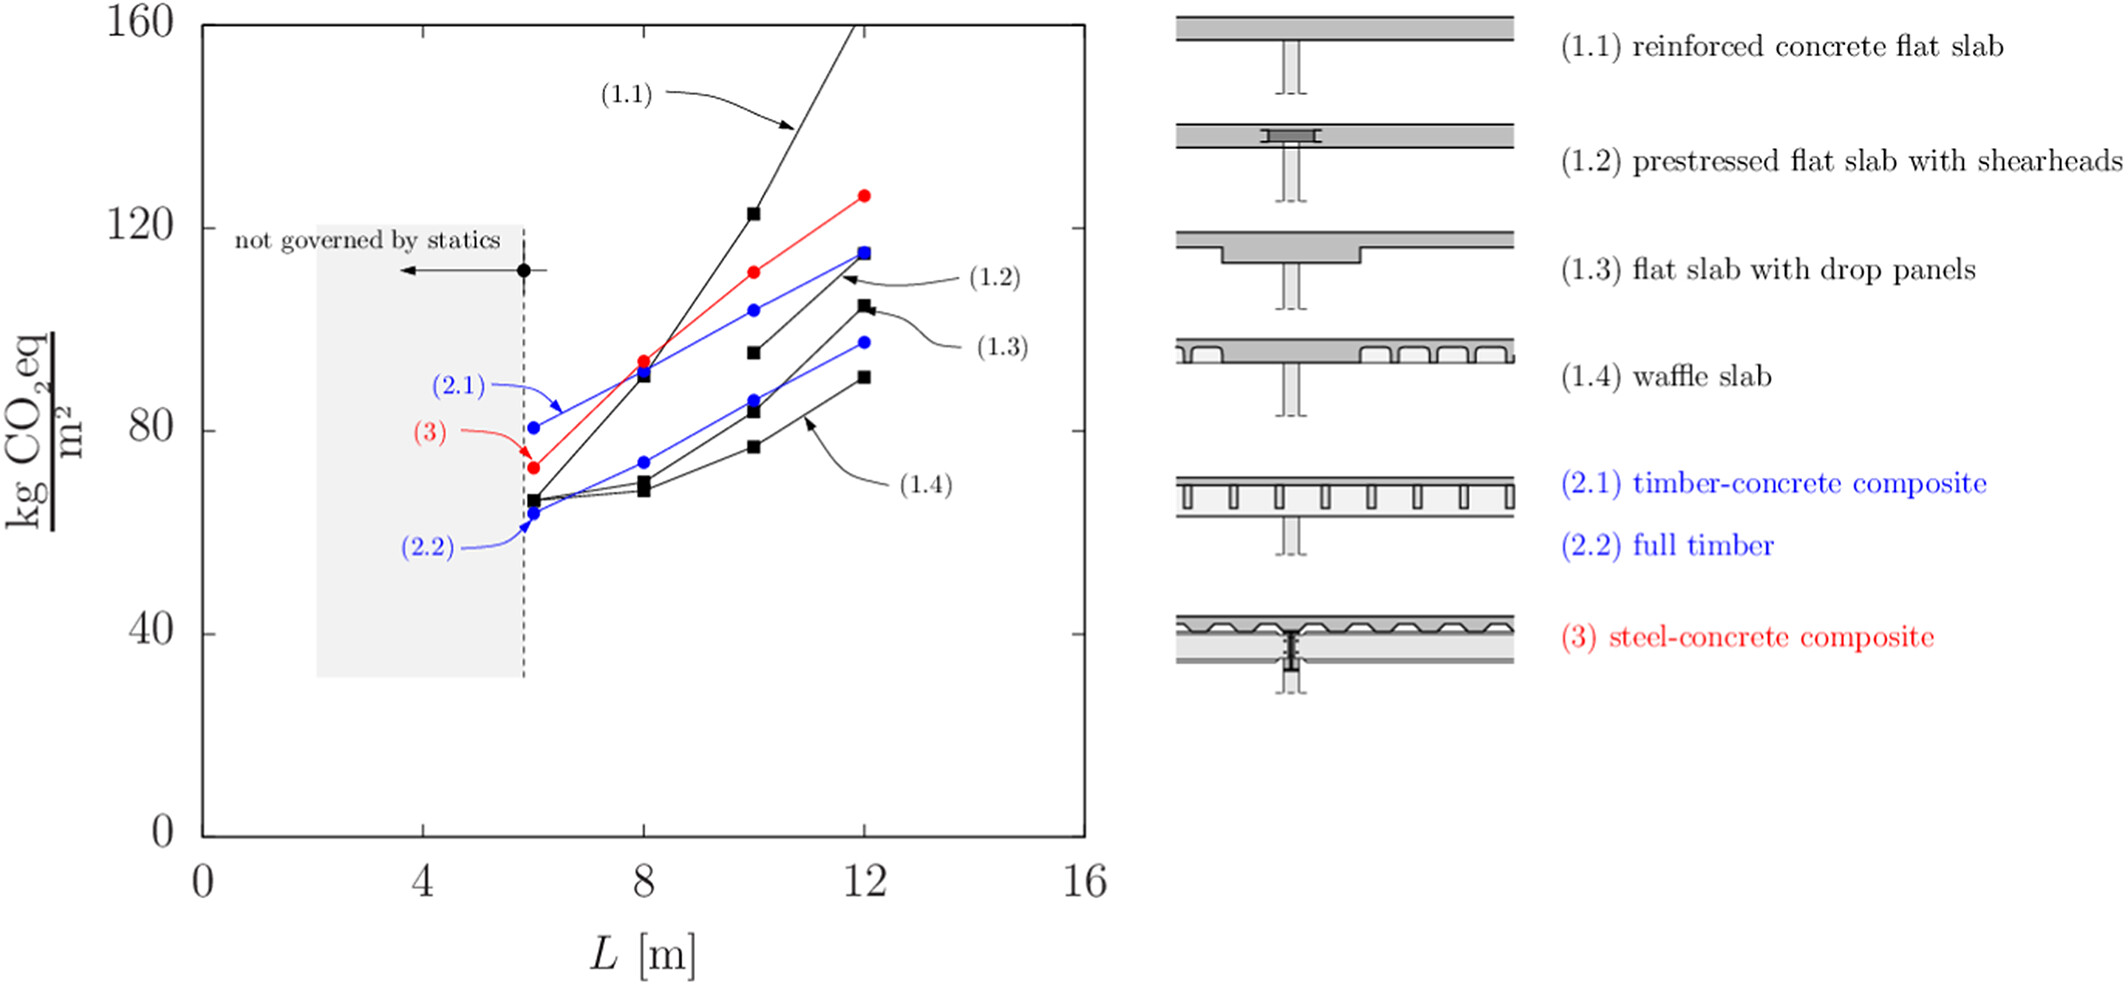
\includegraphics[width=0.7\textwidth]{figures/sustainability2022.jpg}
    \caption{Calculated embodied CO$_2$eq for the different structural systems, adopted from \citep{RefWorks:regulez2022sustainability}}
    \label{fig:regulez2022}
\end{figure} 

\begin{figure}[h!]
    \centering
    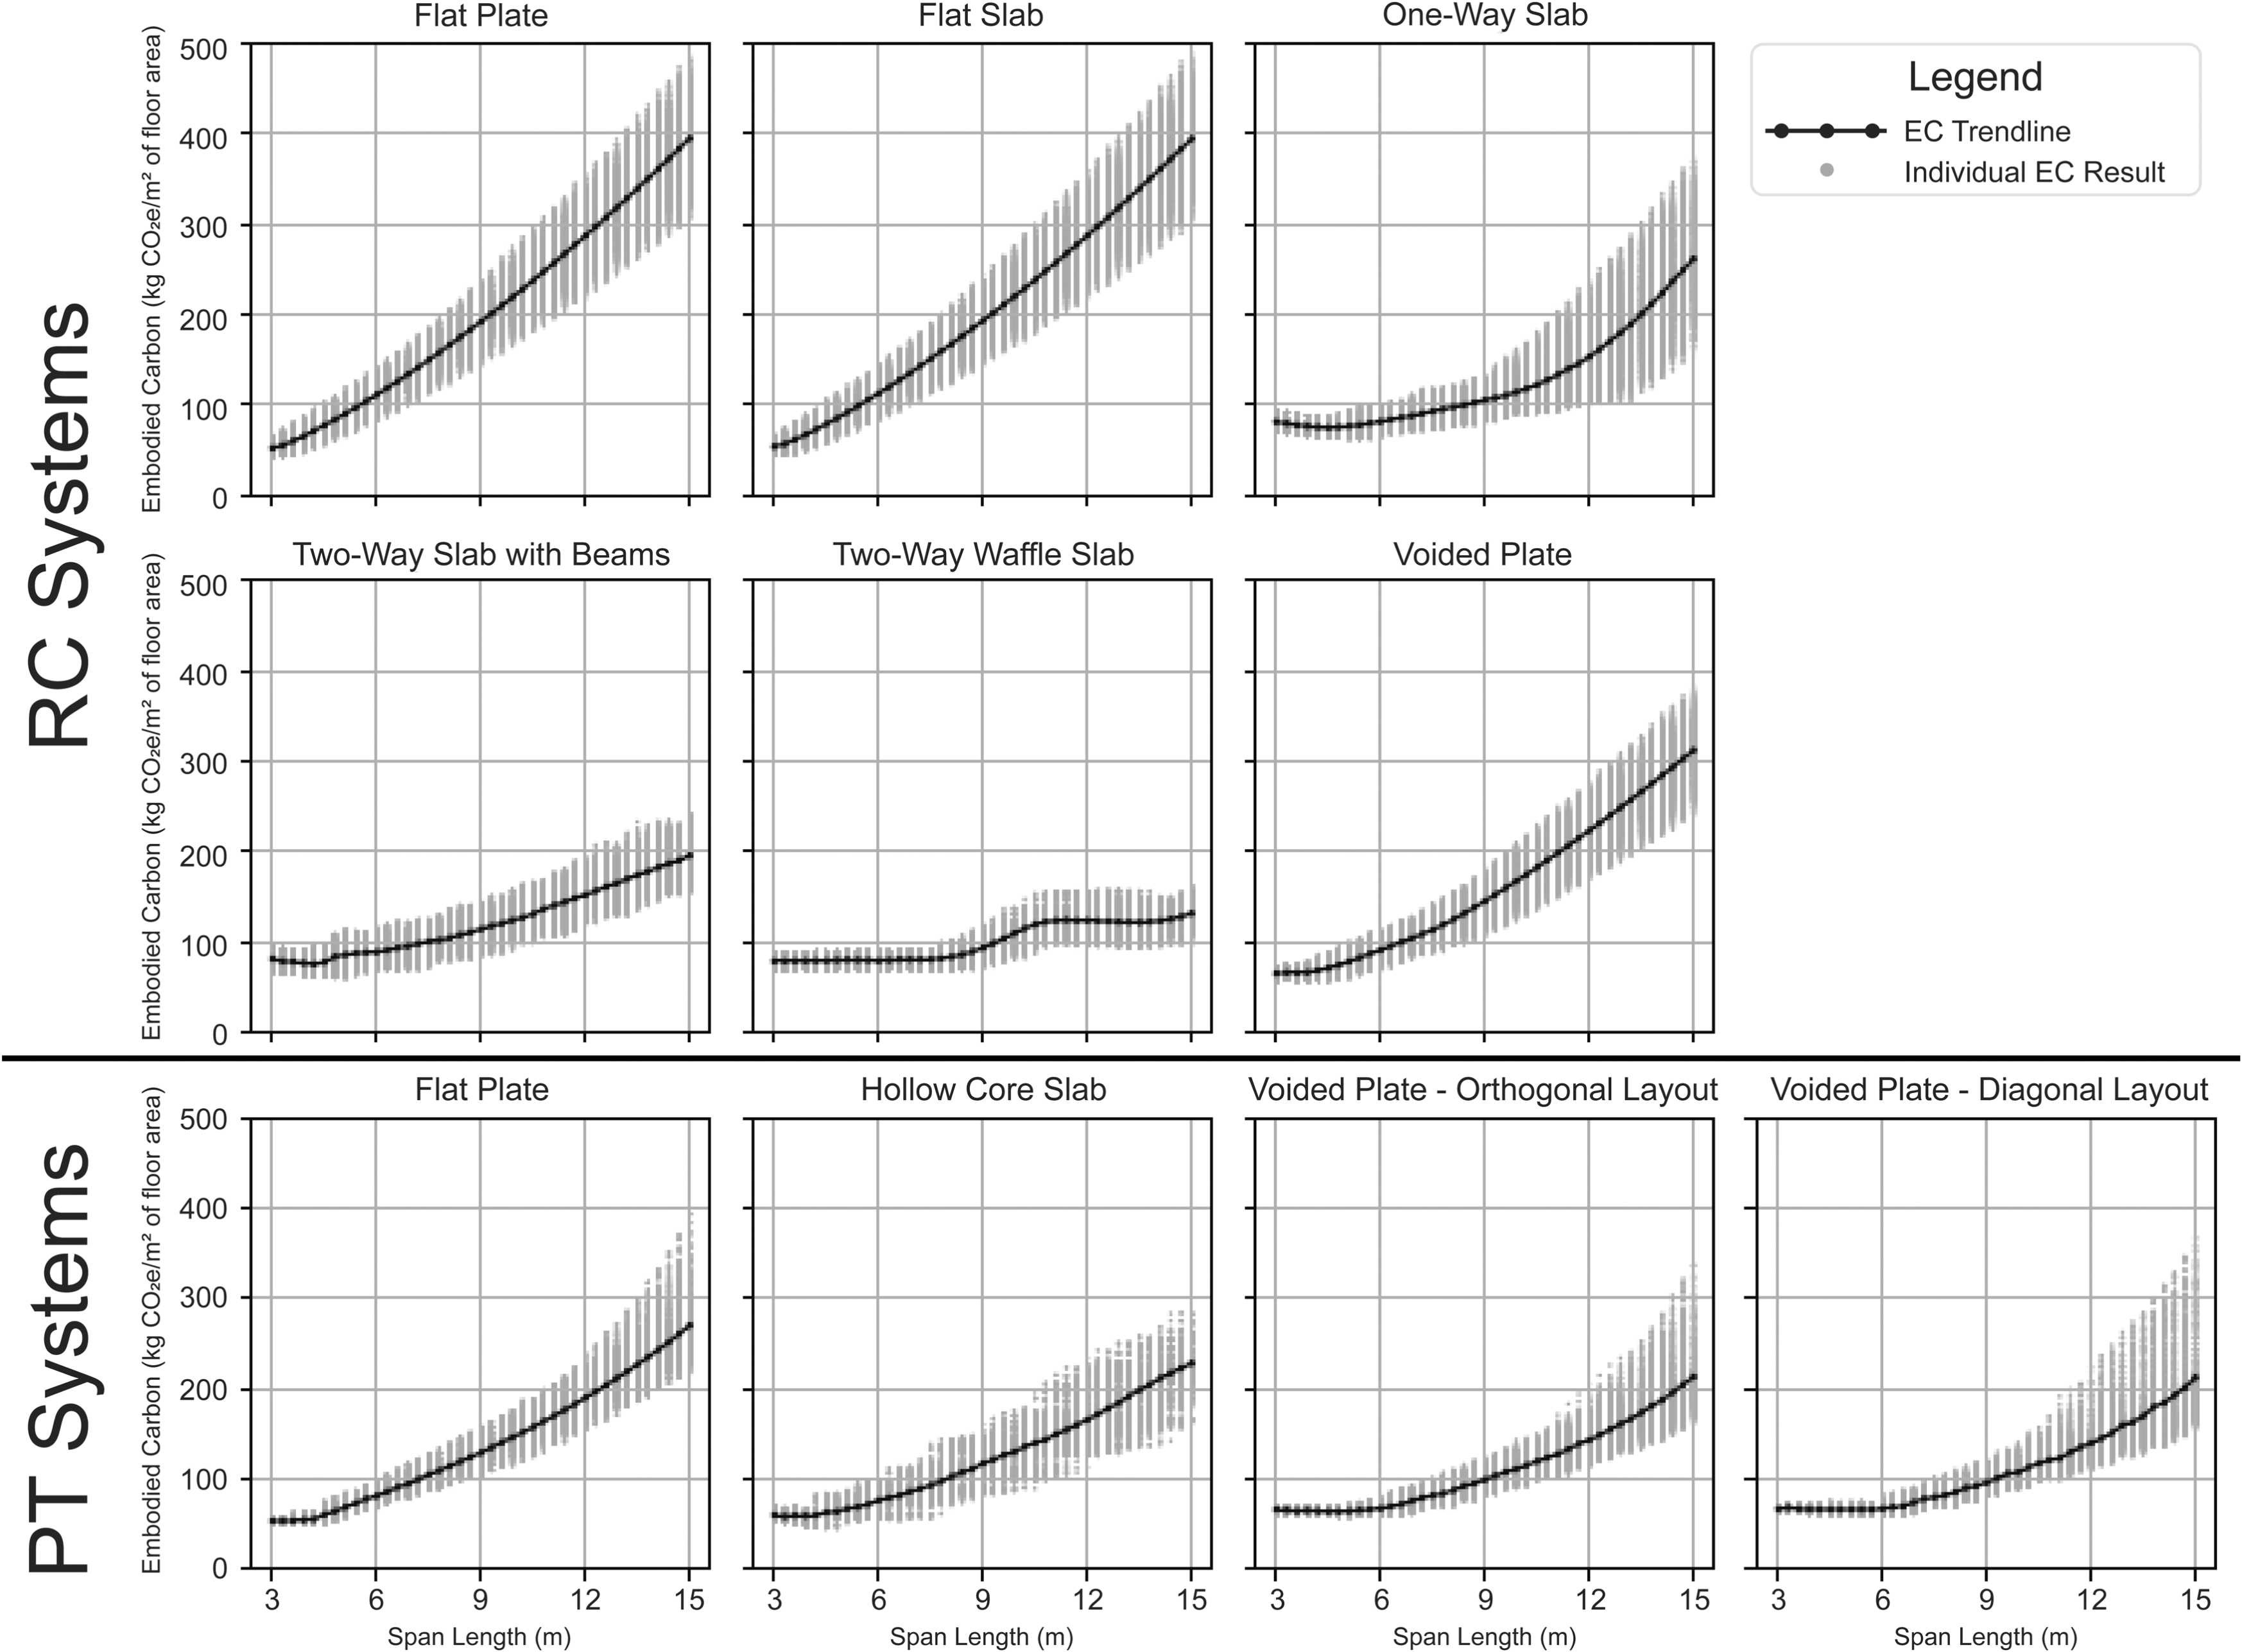
\includegraphics[width=0.7\textwidth]{figures/equations.jpg}
    \caption{The composite EC trendlines superimposed over all simulated results for each system, adopted from \citep{RefWorks:broyles2024equations}}
    \label{fig:broyles2024}
\end{figure} 

While a growing body of research has examined the optimisation of reinforced concrete structures, comparatively little attention has been given to alternative slab typologies such as steel–concrete composite systems. In particular, slim floor systems, which integrate steel beams within the slab depth, offer the potential to reduce structural depth and concrete volume while maintaining structural capacity. However, the environmental implications of these systems remain relatively under explored in comparison to traditional reinforced concrete solutions.

In summary, reducing the embodied carbon of buildings requires greater attention to structural system selection and material efficiency during early-stage design. Life Cycle Assessment and Global Warming Potential provide useful metrics for evaluating the environmental performance of structural materials and systems. Although optimisation techniques have increasingly been applied to reinforced concrete structures, the environmental performance of composite slab systems such as slim floor slabs has received comparatively limited investigation. 
%---------------------------------------------------------------
\subsection{Development of Composite Slabs}
%---------------------------------------------------------------
Composite construction combines steel and concrete elements so that they act together structurally as a single unit. The purpose of this configuration is to exploit the mechanical properties of each material: steel provides high tensile strength and stiffness, while concrete performs well in compression and offers inherent fire resistance and durability. When these materials are effectively connected, the resulting structural element can achieve higher strength and stiffness compared with the individual components acting independently \citep{RefWorks:ahmed2019evolution}.

The concept of composite construction emerged in the late nineteenth century with early applications of concrete-encased steel beams, such as bridge structures constructed in Pittsburgh in 1894 \citep{RefWorks:ahmed2019evolution}. At this stage, concrete primarily served as fire protection rather than as a structural component. However, during the mid-twentieth century researchers began recognising the structural advantages of enabling concrete slabs to participate in resisting bending forces together with steel beams. The development of welded headed shear studs in the 1950s represented a key technological breakthrough, allowing effective transfer of longitudinal shear forces between steel and concrete and thereby enabling reliable composite action \citep{RefWorks:ahmed2019evolution}.

During the same period, the introduction of profiled steel decking significantly accelerated the adoption of composite floor systems in building construction, with mesh reinforcement being welded to the surface of a standard decking profile \citep{RefWorks:widjaja2000developments}. Metal decking functions both as permanent formwork during construction and as tensile reinforcement in the completed slab. This dual functionality eliminates the need for traditional formwork while providing a working platform during construction, thereby improving construction speed and efficiency \citep{RefWorks:composite}. The decking also provides lateral restraint to steel beams during the construction stage, which further simplifies erection procedures.

Composite slabs typically consist of in-situ reinforced concrete cast onto profiled steel decking. The decking profiles may be trapezoidal or re-entrant in shape, with depths commonly ranging from 50–80 mm for shallow decking and up to 225 mm for deep decking systems. Force is transferred via embossments and indentations as well as the deck geometry. Additional reinforcement bars may be placed  within the decking troughs, particularly for concentrated loads or for fire resistance requirements \citep{RefWorks:johnson2018composite}. In many cases, the decking can span between beams without temporary propping during construction, with typical unpropped spans ranging from approximately 4.5 m for shallow profiles to around 6 m for deep decking systems \citep{RefWorks:ahmed2019evolution}.

\begin{figure}[h]
\begin{subfigure}{0.5\textwidth}

\includegraphics[width=0.9\linewidth, height=5cm]{figures/reentrant.png} 
\caption{reentrant}
\label{fig:reentrant}
\end{subfigure}
\begin{subfigure}{0.5\textwidth}

\includegraphics[width=0.9\linewidth, height=5cm]{figures/trapezoidal.png}
\caption{trapezoidal}
\label{fig:trapezoidal}
\end{subfigure}
\caption{Types of steel decking profiles in composite slabs \citep{RefWorks:composite}}
\label{fig:steeldeckings}
\end{figure}

In conventional composite floor construction, the steel beam is located below the slab and supports the composite slab through welded shear studs. This arrangement is known as the downstand composite beam, which remains the most common type of composite beam used in steel-framed buildings \citep{RefWorks:ahmed2019evolution}. The composite action between the two materials increases the bending resistance of the beam and significantly improves stiffness compared with a non-composite steel section. Composite action between the slab and the beam is achieved through headed shear studs, attached to the upper flange of the steel beam with a process called through deck welding \citep{RefWorks:composite}.

The widespread adoption of composite floor systems has been driven by several advantages. Composite construction reduces the self-weight of structural elements, which in turn decreases the loads transferred to columns and foundations. Additionally, the use of steel decking reduces construction time and simplifies site operations by minimising the need for formwork and temporary supports \citep{RefWorks:lawson1999slimflor}. As a result, composite construction has become a dominant structural solution in multi-storey steel buildings, especially in the UK for non-residential projects.

Despite these advantages, conventional downstand composite beams present certain limitations. Because the steel beam is positioned below the slab, the overall structural depth of the floor system can be relatively large. Increasing span lengths further increases beam depth, which can lead to inefficient structural proportions and increased steel consumption \citep{RefWorks:hicks2003current}. Furthermore, welding shear studs on site and waiting for in-situ concrete to cure can introduce additional construction time and cost. These limitations have motivated the development of alternative floor systems that integrate the beam within the slab depth - known as slim floor construction.

%---------------------------------------------------------------
\subsection{Commercial Slim Floor Systems} \label{sec:commercial_slim_floor}
%---------------------------------------------------------------
Slim floor systems were introduced in the early 1990s as an alternative to conventional downstand composite beams \citep{RefWorks:ahmed2019evolution}. In these systems, the steel beam is integrated within the thickness of the floor slab rather than placed below it. This configuration allows the underside of the slab to remain flat, producing what is commonly referred to as a flat soffit. The flat soffit simplifies the installation of mechanical and electrical services and provides greater architectural flexibility for building layouts.

By incorporating the steel beam within the slab depth, slim floor systems can significantly reduce floor-to-floor height while maintaining the required structural capacity. Reductions in storey height of approximately 300 mm are commonly achievable compared with traditional downstand beam systems \citep{RefWorks:lawson2015slimfloor}. Over the height of a multi-storey building, these reductions can lead to substantial savings in façade materials and building envelope costs, or alternatively allow additional floors to be constructed within a fixed building height. Unlike standard slabs that sit on the top flange, slim floor units are supported on the bottom flange or a welded plate. This places the beam web in a state of partial encasement, which provides inherent lateral-torsional restraint.

Slim floor systems are particularly attractive for building types where floor depth and service integration are critical design considerations, such as residential buildings, hospitals, and office developments \citep{RefWorks:lawson2015slimfloor}. In addition to architectural benefits, the partial encasement of steel beams within concrete can improve fire performance, with many slim floor systems achieving up to 60 minutes of fire resistance without additional protection \citep{RefWorks:lawson1999slimflor}. This is because the majority of the steel section is encased in concrete, the concrete acts as a heat sink, protecting the steel web and top flange.

One popular commercial system is ArcelorMittal's slim floor which consists of a rolled steel section with a plate welded to the bottom flange which acts as a shelf to support either precast concrete floor units or deep composite decking \citep{RefWorks:arcelormittal2017slimfloor}. In this case, the beam section is known as a 'SlimFlor' beam. Shear studs are often used to provide composite action and result in a span of between 5-10 m with structural depths between 280 and 320 mm \citep{RefWorks:lawson1999slimflor}.  An example of the slim floor system is shown in Figure~\ref{fig:slimflor}. The range of deep steel decking manufactured by ArcelorMittal is called Cofraplus, however they also produce Cofradal, a prefabricated slab consisting of a metal deck and an insulation layer.

Several variations of slim floor beams have since been developed in an attempt to improve structural performance. One such variation is the Asymmetric Slim-floor Beam (ASB), which uses a rolled beam with thick asymmetric flanges \citep{RefWorks:rackham2006design} to enhance the torsional stiffness. The top flange is also embossed to help provide the composite action between the steel beam and the concrete slab without the need for shear studs. ASB systems can typically reach spans between 6-7.5m with a depth of 310-340mm \citep{RefWorks:ahmed2019evolution}. They can also achieve 90 minute fire resistance, higher than the 60 minute resistance of slim floor beams \citep{RefWorks:bailey1999behaviour}. There is, however, little research on the vibration response of these systems. The ASB shown in Figure~\ref{fig:slimdek}, was developed for use with ComFlor 225 deep decking to form the 'SlimDek' floor system developed by Tata Steel. Tata Steel are a manufacturer of steel and have a range of composite floor deck profiles, known as ComFlor, for both downstand and slim floor beam construction.

\begin{figure}[h]
\begin{subfigure}{0.49\textwidth}
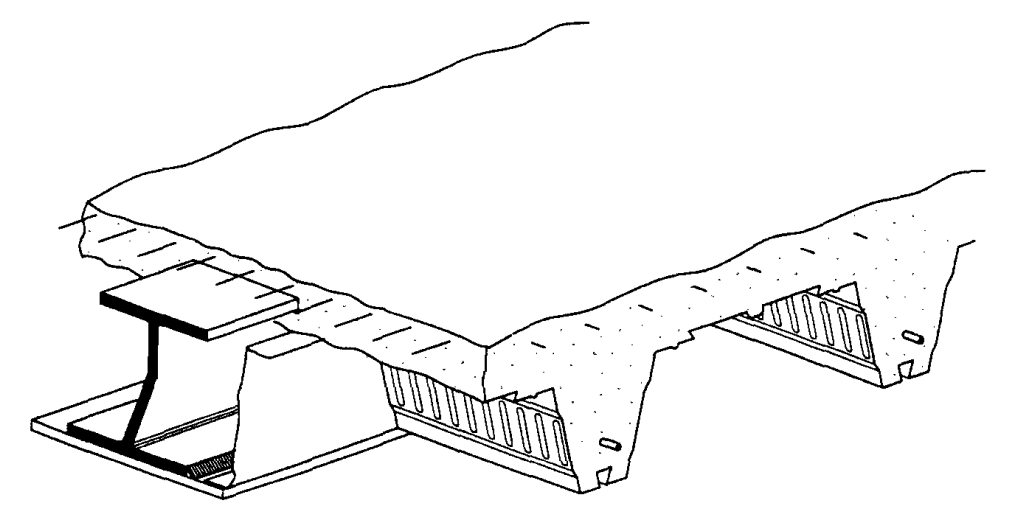
\includegraphics[width=\textwidth, height=5cm]{figures/slimflor.png} 
\caption{SlimFlor beam}
\label{fig:slimflor}
\end{subfigure}
\begin{subfigure}{0.49\textwidth}
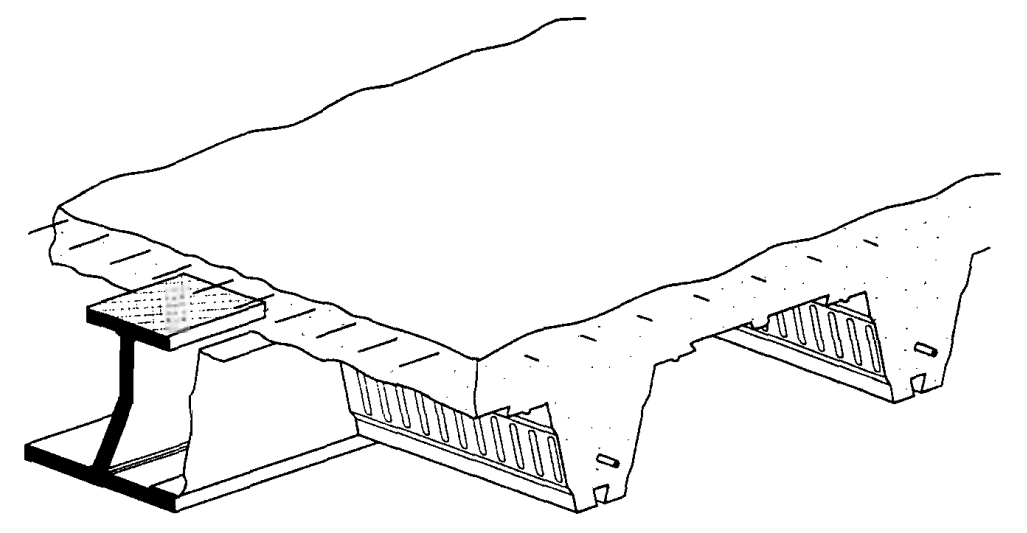
\includegraphics[width=\textwidth, height=5cm]{figures/slimdek.png}
\caption{SlimDek floor system}
\label{fig:slimdek}
\end{subfigure}
\caption{SlimFlor vs SlimDek (ASB) systems \citep{RefWorks:lawson1999slimflor}}
\label{fig:slimfloorvsasb}
\end{figure}

Aside from the basic slim floor system, many manufacturers have created their own systems that either change the beam section or shear connection to achieve different structural performances. \cite{RefWorks:arcelormittal2017slimfloor} introduced the Composite Slim Floor Beam (CoSFB) as a new development into improving shear transfer between the steel beam and the surrounding concrete. This system uses web opening in the steel beam to allow concrete to pass through the web, forming concrete dowels that provide shear connection between the beam and the slab. It also increases the allowable span from approximately 10 to 12 m while also reducing the slab depths compared to standard slim-floor beams \citep{RefWorks:ahmed2019evolution}. The CoSFB system can also be used with the Cofradal slab system as well as standard steel decking.
 
\cite{RefWorks:2024deltabeam} developed the DELTABEAM system which consists of a hollow steel box section with regularly spaced web openings. Similar to CoSFB, concrete passes through these openings to enable composite action. This system can achieve a span of 13.5 m with a structural depth of 500 mm and can achieve a fire resistance of 60 minutes and vibration performance of 3 Hz but more studies are required due to the configuration complexity \citep{RefWorks:peltonen2012connection}.

\cite{RefWorks:ju2003structural} researched a new type of slim floor beam known as i-TECH beams. It consisted of an asymmetric steel beam with web openings, formed through welding a top plate to a bottom tee-section. Non-structural channels are also fixed to the bottom flange of the steel beam to support the deck. Instead of using shear connectors, composite action is achieved through the bond strength of the interface between the concrete slab and the steel beam. The beam can span from 7.5 to 15m with a depth of 300mm however it only reaches a fire resistance of 40 minutes which is less than that provided by SlimFlor  beams \citep{RefWorks:ju2009flexural}.

Another example is the Ultra Shallow Floor Beam (USFB) developed by Westok. This system consists of two asymmetric tee-sections welded together to form a cellular beam with web openings. Similar to other recent systems, composite action is achieved through concrete dowel connections. It is also recommended to provide rebars within the openings to improve the continuity of the slabs on either side of the beam \citep{city1965}. USFB systems can achieve spans of up to 10 m with a depth of 300 mm, outperforming the other shallow floor beams presented \citep{RefWorks:ahmed2019evolution}.

\begin{figure}[h]
 \begin{subfigure}{0.49\textwidth}
     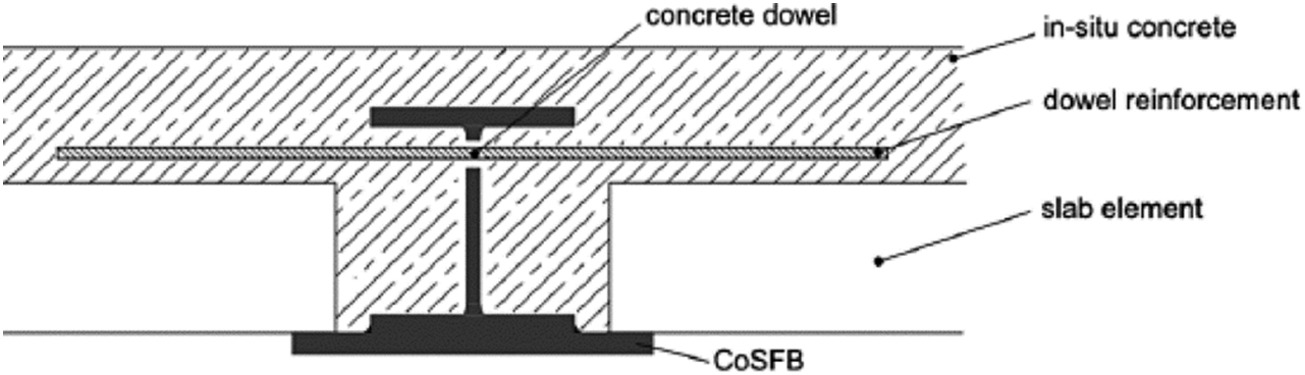
\includegraphics[width=\textwidth]{figures/Cosfb.jpg}
     \caption{CoSFB}
     \label{fig:cosfb}
 \end{subfigure}
 \hfill
 \begin{subfigure}{0.49\textwidth}
     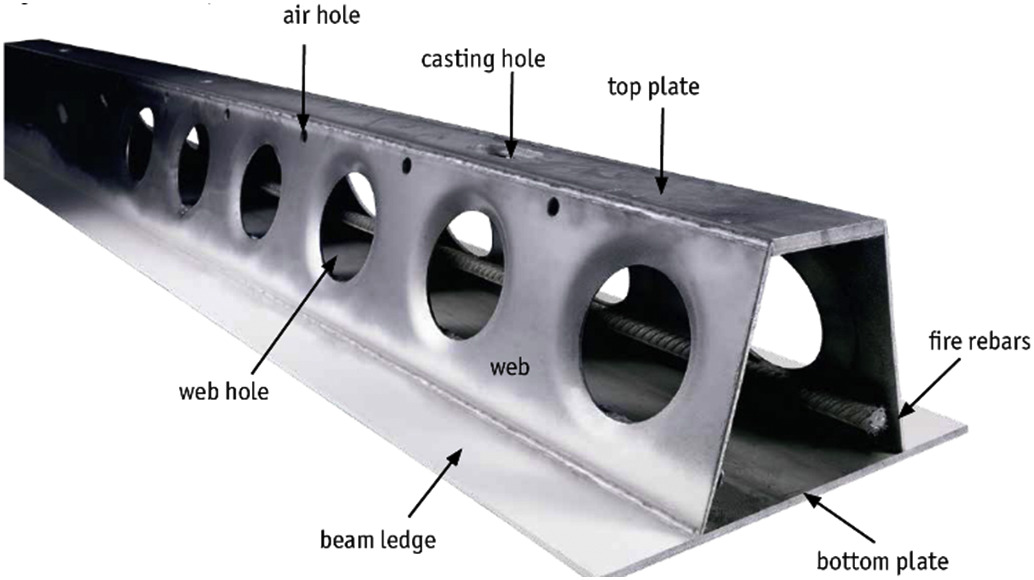
\includegraphics[width=\textwidth]{figures/deltabeam.jpg}
     \caption{DELTABEAM}
     \label{fig:delta}
 \end{subfigure}
 
 \medskip
 \begin{subfigure}{0.49\textwidth}
     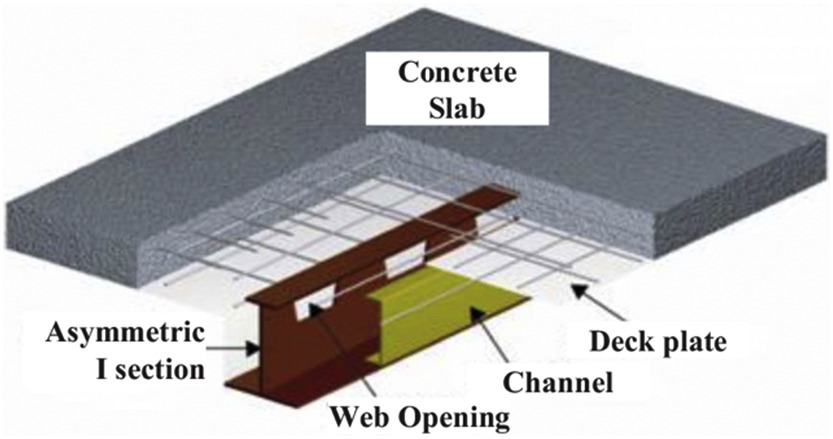
\includegraphics[width=\textwidth]{figures/itech.jpg}
     \caption{ITECH}
     \label{fig:itech}
 \end{subfigure}
 \hfill
 \begin{subfigure}{0.49\textwidth}
     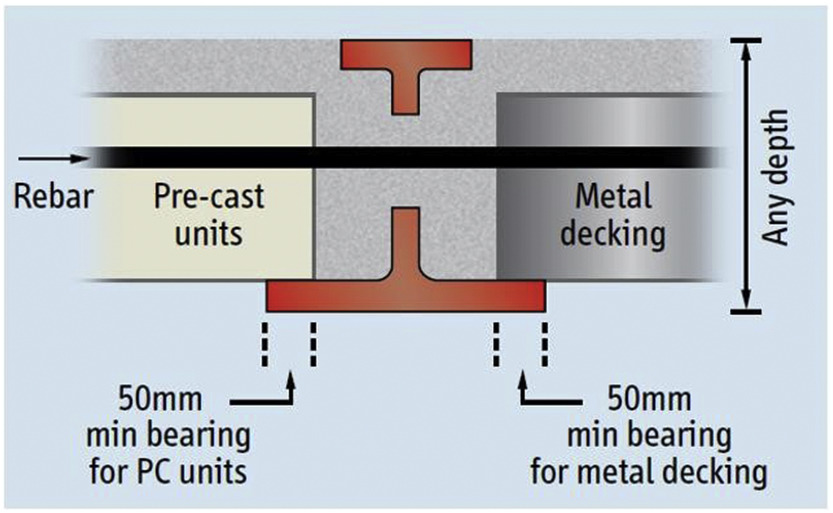
\includegraphics[width=\textwidth]{figures/USFB.jpg}
     \caption{USFB}
     \label{fig:usfb}
 \end{subfigure}

 \caption{Recent developments in Slim-floor systems, adopted from \citep{RefWorks:ahmed2019evolution}}
 \label{fig:advanced slimfloor}
\end{figure}

\begin{table}[h]
\centering
\scriptsize
\caption{Flooring system types, adopted from \citep{RefWorks:ahmed2019evolution}}
\label{tab:slimfloor_comparison}
\begin{tabularx}{\textwidth}{p{2cm}XXXXXXX}
\toprule
 & Composite downstand beam & SlimFlor beam & ASB & ITECH & DELTABEAM & USFB & CoSFB \\
\midrule

Type of shear connection &
Shear stud connection &
Shear stud connection &
Using top flange embossment connections &
Bearing concrete passing through the web opening shear connection &
Bearing concrete passing through the web opening shear connection &
Plug composite action shear connection &
Concrete dowel shear connection \\

Span limitation (m) &
4-6 with metal deck; 6-12 with HCU &
5-10 &
6-7.5 &
7.5-15 &
Up to 13.5 &
Up to 10 &
Up to 12 \\

Depth limitation (mm) &
steel depth + (120-160) mm slab depth &
280-320 &
310-340 &
300 and $>$300 &
200-500 &
300 &
350 \\

Fire performance (min) &
30-240 &
60 &
90 &
40 &
60 &
40 &
60 \\

Vibration performance (Hz) &
N.A.$^\dagger$ &
N.A.$^\dagger$ &
N.A.$^\dagger$ &
$>3$ &
$>3$ &
$>3$ &
$>3$ \\

\bottomrule
    \end{tabularx}
    \vspace{4pt}
    {\footnotesize
    $^\dagger$ Vibration performance figures are not published in
    standard tabular form for conventional downstand composite
    beams, SlimFlor beams, or ASB systems; assessment is carried
    out using a calculation-based approach per \citet{RefWorks:hicks2009p354}.
    The published $>3$~Hz values for ITECH, DELTABEAM, USFB,
    and CoSFB are minimum natural frequency targets drawn from
    manufacturer technical documentation.
    }
\end{table}

These developments demonstrate the ongoing research into slim floor construction, with the aim being to optimise structural performance while reducing construction depth and improve constructibility. The systems discussed are summarised in Table~\ref{tab:slimfloor_comparison} and Figure~\ref{fig:advanced slimfloor}. Although there is a large number of slim floor systems that have been developed, not all are equally suitable for inclusion in the optimisation tool. In particular, complex systems such as DELTABEAM and iTECH rely on non-standard beam geometries which can limit the availability of publicly accessible design tables and product properties needed for implementation. In contrast, systems such as the standard slim floor and 'SlimDek' are based largely on standard hot rolled steel sections which makes the structural behaviour and design procedures easier to implement. 

Another important consideration is the availability of environmental data required for the sustainability objective. Three manufacturers are currently represented in the database: Tata Steel (ComFlor range), ArcelorMittal (Cofraplus range), and Kingspan (Multideck range). All three provide published EPDs and comprehensive design data through technical manuals or proprietary software \citep{RefWorks:2017comflor, RefWorks:2021floors, RefWorks:kingspan2026multideck}. These datasets allow the GWP contribution of each deck product to be quantified from verified manufacturer data. It should be noted, however, that the granularity of available EPD data varies between manufacturers: Tata Steel provide individual declarations for each \mbox{ComFlor} profile, whereas ArcelorMittal and Kingspan each publish a single EPD covering their entire decking range. The implications of this for the environmental assessment are discussed further in Chapter~\ref{thirdchapter}.

Furthermore, SlimFlor beam and SlimDek floor systems have been used in European steel-framed construction and are supported by comprehensive design guidance and technical manuals published by the manufacturers. The availability of established design methods makes these systems particularly suitable for parametric analysis and optimisation. For these reasons, this research focuses primarily on composite downstand, SlimFlor and SlimDek floor systems. The following section therefore reviews the structural design procedures used for composite slabs and slim floor systems, which form the basis of the optimisation methodology developed in this study.
%---------------------------------------------------------------
\subsection{Design Methods}
%---------------------------------------------------------------
The design of composite steel-concrete slabs is governed by the interaction between steel and concrete under both construction and composite loading conditions. In European practice, the design of composite steel and concrete structures is carried out in accordance with Eurocode 4 \citep{RefWorks:cen2004en4}, used alongside Eurocode 2 \citep{RefWorks:cen2004en2} for concrete elements and Eurocode 3 \citep{RefWorks:cen2005en3} for structural steel components. The Eurocodes are a series of standards providing design rules for all common structure types; they are referenced in this report as, for example, 4-1-1/9.4, meaning Clause 9.4 of EN 1994-1-1.

Composite floor systems must be verified for both ultimate limit states (ULS) and serviceability limit states (SLS, comprising crack control, deflection, and vibration), as well as for fire resistance and acoustic performance. A defining feature of their design is its staged nature, which requires the verification of two distinct conditions: the construction stage, in which the wet concrete is supported by the bare steel deck acting as formwork, and the final composite stage, in which the hardened concrete and the deck act together. A further complication is that, in practice, design resistances are frequently derived from manufacturer test data rather than by calculation alone, since the local buckling behaviour of thin profiled sheeting is difficult to capture analytically.

\subsubsection*{Construction stage}
During the construction stage the concrete has not yet hardened and therefore does not contribute to the resistance of the slab; this is often the limiting stage of the design. The steel deck must carry the wet concrete, construction loads, and its own self-weight while acting as falsework. Where deck deflections become significant, an additional load due to ponding of the wet concrete must be considered. Two construction methods are possible. In \textit{unpropped} construction the deck spans unsupported between beams, and for continuous decks the support moments may be partially redistributed into the span. In \textit{propped} construction temporary props carry the wet concrete, permitting thinner slabs and lighter deck profiles, but at the expense of slower construction; in this case no moment redistribution at ULS is permitted \citep{RefWorks:hicks2008en}. The bending, shear, and deflection resistances of the bare deck are specified in Eurocode 3, although manufacturers commonly publish test-derived resistances determined in accordance with EN~1993-1-3 Annex~A, which are less conservative than the analytical effective-width approach.

\subsubsection*{Composite stage}
Once the concrete has hardened, the slab and deck act compositely through longitudinal shear transfer at the steel--concrete interface. The composite section benefits from greatly increased stiffness and bending resistance. The degree of shear connection governs whether full or partial composite action develops; full connection is generally only achievable at longer spans, with the shear bond often being the critical mechanism at shorter spans, in which case only partial composite action is mobilised. Eurocode 4 provides plastic stress-block methods for the sagging moment resistance under both full and partial shear connection.

The longitudinal shear resistance at the steel--concrete interface is assessed using empirical methods, since it cannot be reliably predicted analytically. Two approaches are recognised: the m--k method and the partial connection method. Both rely on standardised slab tests in which the specimens are first cycled to remove the chemical bond, leaving only the mechanical and frictional interlock, and then loaded to failure \citep{RefWorks:stark1990plastic}. The partial connection method yields a characteristic shear bond strength $\tau_{u,Rk}$, whereas the m--k method establishes two empirical constants, $m$ and $k$, representing the mechanical and frictional interlock respectively, from a linear regression of two groups of tests \citep{RefWorks:porter1976design}. \citet{RefWorks:bode1993modern} note several deficiencies of the m--k approach: it is not based on a mechanical model and is therefore less flexible than the partial connection method, its constants conflate all influencing parameters such that they cannot be separated, and it cannot quantify the benefit of additional reinforcement. The shear connection may be enhanced by end anchorage, either by welded headed studs or by deformation of the deck ends, although Eurocode 4 provides design rules only for through-deck welded studs (4-1-1/9.7.4); in practice such connectors are seldom credited in manufacturer design tables, giving a conservative result.

Vertical shear and, where concentrated loads are present, punching shear are verified using the Eurocode 2 provisions for the concrete section, treating the deck and any additional support reinforcement as tensile reinforcement. Serviceability is frequently the controlling consideration for floor slabs: deflection and vibration limits, specified by Eurocode 4 and the relevant National Annex, often govern the final design, particularly at longer spans. The specific limits, partial factors, and the detailed procedures adopted in the present model are set out in Chapter~\ref{thirdchapter}.

\subsubsection*{Vibration}
The principal UK guidance for assessing the vibration serviceability of composite floors is SCI~P354 \citep{RefWorks:hicks2009p354}, which adopts a response-factor approach based on the dynamic response of the floor to walking excitation. The method first determines the fundamental natural frequency $f_0$ of the floor system, accounting for the combined stiffness and mass of the slab and its supporting beams. Floors are then classified by this frequency: \emph{low-frequency} floors (typically $f_0 \lesssim 10$\,Hz) are susceptible to resonance, in which successive footfalls coincide with a harmonic of the walking rate and the response builds up over time, whereas \emph{high-frequency} floors respond transiently to each individual footfall as a series of decaying impulses. A minimum frequency of around 3\,Hz is generally required to avoid the most onerous resonant behaviour.

For each case, the method estimates the modal mass participating in the governing mode, derived from the effective floor area mobilised by the walking path, the floor mass per unit area, and the damping ratio $\zeta$ (taken from tabulated values according to occupancy and fit-out, SCI~P354 Table~4.1), and from this computes the root-mean-square acceleration response to a representative walking force. The acceleration is expressed as a dimensionless response factor $R$, defined relative to the baseline human perception threshold for vertical vibration in BS~6472, and is compared against limiting values that depend on the use of the space (for example, $R \le 8$ for general offices, with stricter limits for sensitive environments). Because the method requires bay-level inputs --- secondary and primary beam spans, bay width, number of adjacent bays, and damping --- that fall outside the scope of a slab-only optimisation, only an indicative slab-alone natural frequency check is incorporated in this study, as discussed in Chapter~\ref{thirdchapter}.

\subsubsection*{Acoustic performance}
Acoustic performance is a further design requirement for floor systems. The two phenomena of concern are airborne sound transmission and impact sound transmission. Single-number ratings are derived from frequency-band measurements in accordance with \citet{RefWorks:isoEN7171} (airborne) and \citet{RefWorks:isoEN7172} (impact), and may be predicted from element performance data using \citet{RefWorks:en12354}. Airborne insulation can be expressed either as the weighted (apparent) sound reduction index $R_\mathrm{w}$ ($R'_\mathrm{w}$ in situ), which characterises the element itself, or as the weighted standardised level difference $D_\mathrm{nT,w}$, which is a field quantity that also accounts for the geometry of the receiving room. Impact sound is rated by the weighted standardised impact sound pressure level $L'_\mathrm{nT,w}$. Spectrum adaptation terms ($C$, $C_\mathrm{tr}$, $C_\mathrm{i}$) may be added to emphasise particular source spectra, $C_\mathrm{tr}$ in particular penalising poor low-frequency performance.

Performance requirements and the descriptors used to express them vary between national standards and intended use. In the United Kingdom, Approved Document~E to the Building Regulations \citep{RefWorks:adePartE} specifies field-measured requirements for separating floors between new-build dwellings of $D_\mathrm{nT,w} + C_\mathrm{tr} \geq 45$~dB for airborne insulation and $L'_\mathrm{nT,w} \leq 62$~dB for impact insulation. In Switzerland, SIA~181 \citep{RefWorks:sia181} expresses its requirements using a standardised level difference descriptor and sets them according to a classification of the sensitivity of the receiving space and the noise exposure. For non-residential spaces such as offices, both jurisdictions relax the airborne requirement.

The structural slab provides the primary contribution to airborne sound insulation through its mass per unit area, in accordance with the mass law. Composite slabs using profiled steel decking tend to have lower mass per unit area than solid reinforced concrete slabs of equivalent structural depth, owing to the void volume within the deck ribs. As a result, composite floor systems often require supplementary acoustic treatment --- typically a floating screed over a resilient layer --- to satisfy impact sound requirements and, in higher-specification applications, to meet airborne insulation targets as well \citep{RefWorks:scip300}. Since the acoustic performance of the floor depends heavily on the non-structural build-up layers rather than the structural cross-section alone, the choice of floor build-up in this study is informed by the acoustic requirements of each occupancy scenario, as discussed further in Chapter~\ref{thirdchapter}.

\subsubsection*{Fire resistance}
Fire resistance is a critical design requirement for structural floor systems. Composite slabs and slim floor systems generally perform well in fire owing to the presence of the concrete, but design is still carried out in accordance with Eurocode 4. Slim floor systems offer a particular advantage because the steel beam is partially or fully encased within the concrete slab, which reduces the rate of temperature rise in the steel and can eliminate the need for applied fire protection; ratings of 60 to 90 minutes are commonly achievable without protection, depending on slab thickness and reinforcement \citep{RefWorks:hicks2008en}. EN~1994-1-2 (4-1-2/4.3.1) \citep{RefWorks:cen2005en} governs the fire design of composite slabs, with detailed checks for moment resistance and thermal insulation given in its Annex~D; the UK provides alternative guidance under \citet{RefWorks:francis2013ncci}, on which some manufacturers base their design. Thermal insulation is satisfied by providing a minimum slab thickness that depends on the deck profile (re-entrant or trapezoidal) and the concrete type. Most manufacturers publish fire design tables based on the detailed calculation methods of their home-country standards --- either the Eurocodes or the now-withdrawn British Standards.

\subsubsection*{Manufacturer design resources}
In practice, the design of composite slabs and slim floor systems is strongly supported by manufacturer technical manuals, design tables, and dedicated software, which translate the code rules into practical engineering solutions and are widely used for preliminary design and verification. \citet{RefWorks:2017comflor}, \citet{RefWorks:2021floors}, and \citet{RefWorks:kingspan2026multideck} are examples of manuals providing pre-calculated tables of allowable spans, load capacities, slab depths, reinforcement requirements, and fire ratings for standard configurations, enabling rapid system selection without detailed hand calculation. However, these tables are based on discrete parameter sets, restricting the exploration of non-standard configurations, and proprietary software often limits transparency in the underlying calculations. Both characteristics constrain their use in a custom optimisation framework, where explicit control over input parameters and calculation methods is required --- motivating the transparent, parametric implementation of the design checks developed in this study and described in Chapter~\ref{thirdchapter}.

%---------------------------------------------------------------
\subsection{Synthesis and Research Gaps}
%---------------------------------------------------------------
The literature reviewed in this chapter highlights the increasing importance of reducing embodied carbon within structural design. Structural systems, and in particular floor slabs, represent a significant proportion of the total material consumption in multi-storey buildings and therefore offer substantial potential for reducing environmental impact through improved material efficiency and system selection.

Composite construction has emerged as an effective strategy for improving structural efficiency by combining the advantageous properties of steel and concrete. The development of composite floor systems, including profiled steel decking and shear connection technologies, has enabled widespread adoption in modern construction. More recently, slim floor systems have been developed to further improve structural efficiency by integrating steel beams within the slab depth, reducing overall floor height while maintaining structural performance.

A range of slim floor systems have been identified in the literature, including SlimFlor, SlimDek, CoSFB, and Delta beam systems. These systems offer varying performance in terms of span capabilities, structural depth, and construction efficiency. However, their design is typically supported by manufacturer-specific guidance, technical manuals, and software tools, which are largely based on the design principles outlined in Eurocode standards. While these tools facilitate practical design, they are generally oriented towards discrete design solutions and may limit flexibility when exploring a wider design space.

Although previous research has investigated the optimisation of structural systems with respect to material use and environmental impact, the majority of studies have focused on conventional reinforced concrete slabs. Comparatively limited research has been identified that examines the environmental performance of steel–concrete composite slab systems, and in particular slim floor configurations, within an optimisation framework. Furthermore, existing design tools are not typically structured to directly incorporate environmental performance metrics such as Global Warming Potential into the design process.

Another limitation identified in the literature is the reliance on discrete design tables and proprietary software tools, which restrict the ability to explore continuous design variables and understand the influence of individual parameters. While these tools are effective for practical design, they lack the transparency and flexibility required for parametric optimisation studies. This highlights the need for a more adaptable modelling approach that integrates structural design checks with environmental assessment in a unified framework.

Based on these observations, a clear research gap exists in the development of a parametric and optimisation-based approach for evaluating composite slim floor slab systems with respect to embodied carbon. This research therefore aims to address these gaps by developing a parametric structural model for slim floor slab systems, enabling systematic evaluation and optimisation of their environmental performance. The focus on widely used systems such as SlimFlor and SlimDek ensures that the results remain relevant to current engineering practice while allowing sufficient flexibility for detailed analysis.